\section{Auswertung}
\label{sec:Auswertung}
Der Eigenwiderstand des verwendeten Voltmeters beträgt $R_v=\SI{10}{\mega\ohm}$, dessen systematischer Fehler liegt bei $\num{+-15}\%$, der des Amperemeters beträgt $\num{+-3}\%$.
\subsection{Monozelle und Gegenspannung}
Der wie in der Durchführung beschriebene gemessene Wert für die Leerlaufspannung der Monozelle beträgt $U_{0,\text{mono}} = \SI{1.55}{\volt}$.
Dabei wird der Widerstand $R_a$ jeweils in einem Bereich von $\SI{0}{\ohm}$ bis $\SI{50}{\ohm}$ varriert.
Die Messwerte sind in Tabelle \ref{tab:1} für die Monozelle und in Tabelle \ref{tab:2} für die gegenläufige Schaltung dargestellt.
\begin{table}
  \hspace*{\fill}
  \begin{subfigure}{0.40\textwidth}
  \centering
  \caption{Messdaten Monozelle.}
  \label{tab:1}
  \sisetup{table-format=3.4}
  \begin{tabular}{c c c}
    \toprule
    {$R_a-\text{Wert}$} & {$I [\si{\ampere}]$} & {$U_k [\si{\volt}]$} \\
    \midrule
    \input{build/monotabelle.tex}
    \bottomrule
  \end{tabular}
\end{subfigure}
\hspace*{\fill}
\begin{subfigure}{0.40\textwidth}
  \centering
  \caption{Messdaten Gegenspannung.}
  \label{tab:2}
  \sisetup{table-format=3.4}
  \begin{tabular}{c c c}
    \toprule
    {$R_a-\text{Wert}$} & {$I [\si{\ampere}]$} & {$U_k [\si{\volt}]$} \\
    \midrule
    \input{build/gegentabelle.tex}
    \bottomrule
  \end{tabular}
\end{subfigure}
\\
\hspace*{\fill}
\hspace*{\fill}
\caption{Messdaten für die Monozelle und die Gegenspannung.}
\end{table}

Somit ergibt sich der Monozellenplot in Abbildung \ref{fig:1},

\begin{figure}[H]
  \centering
  \includegraphics[height=8cm]{build/monoplot.pdf}
  \caption{Monozellenplot}
  \label{fig:1}
\end{figure}

sowie der Plot mit der angesetzten Gegenspannung in Abbildung \ref{fig:2}

\begin{figure}[H]
  \centering
  \includegraphics[height=8cm]{build/gegenplot.pdf}
  \caption{Gegenspannungsplot}
  \label{fig:2}
\end{figure}

Beide Ausgleichsgeraden wurden mit numpy auf eine lineare Funktion inklusive Fehlerbalken der Form
\begin{equation}
  f(x) = b + mx
\end{equation}
gefittet, wobei für die Monozelle
\begin{equation}
  U_k(I) = U_0 - R_iI
\end{equation}
und für die gegenläufige Schaltung
\begin{equation}
  U_k(I) = U_0 + R_iI
\end{equation}
gilt.
Zur Berechnung der jeweiligen Leerspannung und des Innenwiderstandes wurde die Methode der linearen Regression,
\begin{align}
  m &= \frac{ n \sum_{i=1}^n x_i y_i - \sum_{i=1}^n x_i \sum_{i=1}^n y_i }{n\sum_{i=1}^n x_i^2 - ( \sum_{i=1}^n x_i )^2}\\
  \notag\\
  b &= \frac{ \sum_{i=1}^n x_i^2 \cdot \sum_{i=1}^n y_i - \sum_{i=1}^n x_i \cdot \sum_{i=1}^n x_i y_i}{n\sum_{i=1}^n x_i^2 - ( \sum_{i=1}^n x_i )^2},
\end{align}
bei $n$ Messwerten, gewählt.
\\
Die Standardabweichungen berechnen sich zu
\begin{align}
  \sigma_m &= \sqrt{ \sigma_y^2 \frac{n}{n \sum_{i=1}^n x_i^2 - (\sum_{i=1}^n x)^2} }\\
  \sigma_b &= \sqrt{ \sigma_y^2 \frac{\sum_{i=1}^n x_i^2}{n \sum_{i=1}^n x_i^2 - (\sum_{i=1}^n x)^2} }
\end{align}
für die Steigung $m$, welche für den Innenwiderstand $R_i$ steht, und für den y-Achsenabschnitt $b$, der die Leerlaufspannung $U_0$ darstellt.%\cite{Walcher}
Daraus folgen die jeweiligen Werte
\begin{align*}
  U_{0,{mono}}  &= \input{build/mono_u0.tex}  & R_{i,mono}  &= \input{build/mono_ri.tex},\\
  U_{0,{gegen}} &= \input{build/gegen_u0.tex} & R_{i,gegen} &= \input{build/gegen_ri.tex}.
\end{align*}





%\begin{figure}
%  \centering
%  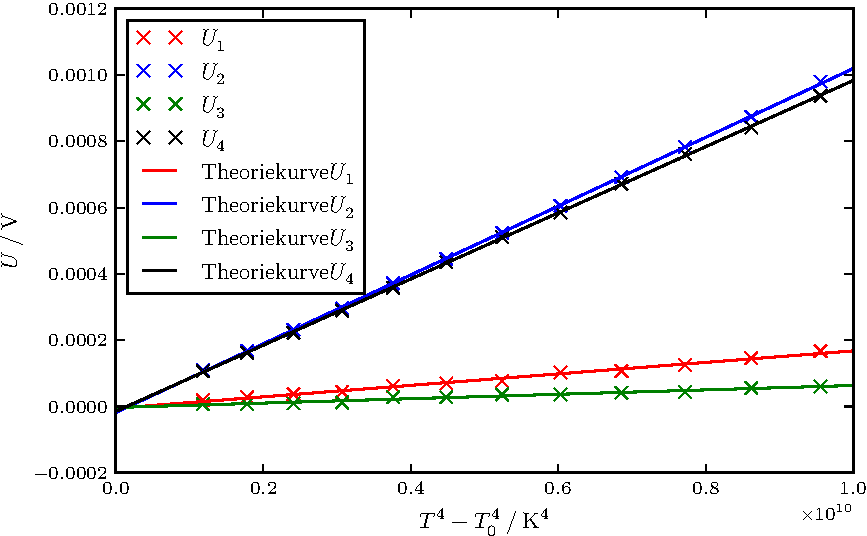
\includegraphics{plot.pdf}
%  \caption{Plot.}
%  \label{fig:plot}
%\end{figure}
%
%\begin{table}
%  \centering
%  \caption{Beispieltabelle}
%  \label{tab:tabelle_beispiel}
%  \sisetup{table-format=1.2}
%  \begin{tabular}{c c}
%    \toprule
%    {$a [\si{\second}]$} & {$b [\si{\kelvin}]$}\\
%    \midrule
%    1.0000  & 11.00 \\
2.0000  & 12.00 \\
3.0000  & 13.00 \\
4.0000  & 14.00 \\
5.0000  & 15.00 \\
6.0000  & 16.00 \\
7.0000  & 17.00 \\
8.0000  & 18.00 \\
9.0000  & 19.00 \\
10.0000 & 20.00 \\

%    \bottomrule
%  \end{tabular}
%\end{table}
%
%Es ergibt sich
%\begin{align}
%  a &= (0 \pm 0) ~ \si{\joule\per\kelvin\per\gram}
 \\
%\end{align}
